\hypertarget{handel}{%
\chapter{Handel}\label{handel}}

\begin{blockquotebox}
    De essentiële inzichten die de basis vormden voor samenwerking, maatschappij en beschaving\index{beschaving}, en die de mens boven zijn dierlijke oorsprong uit tilden, omvatten het besef dat arbeid, wanneer verricht in het kader van arbeidsdeling\index{arbeidsdeling}, productiever is dan individueel verrichte arbeid, en dat het menselijk intellect in staat is deze realiteit te erkennen.\footnotemark
    \par\raggedleft--- Ludwig von Mises\index{Ludwig von Mises}
\end{blockquotebox}
\footautocite{105}

In de voorgaande hoofdstukken hebben we besproken hoe economische handelingen en ruiltransacties kunnen plaatsvinden in afzondering. Arbeid, kapitaalaccumulatie en technologische innovaties in productieprocessen zijn allemaal taken die mensen kunnen gebruiken om hun welzijn te verbeteren zonder interactie met anderen. Ze kunnen arbeid inruilen voor vrije tijd, uitgestelde voldoening inruilen voor directe voldoening en nieuwe technologieën voor oude. Maar mensen zijn sociale dieren, geboren in een familie en een uitgebreide sociale orde, en ze brengen hun leven door in interactie met anderen. Handel drijven met anderen is een instinctief en natuurlijk onderdeel van het leven, iets wat kinderen al op jonge leeftijd doen. De economisch\index{economisch} meest opvallende manier waarop mensen met elkaar kunnen omgaan is door middel van handel of vrij ruilverkeer. In dit hoofdstuk worden de beweegredenen en voordelen van vrij ruilverkeer onderzocht en uitgelegd. De volgende hoofdstukken bouwen hierop voort om een completer beeld te ontwikkelen van onpersoonlijk ruilverkeer in de monetaire marktorde.

Het uitwisselen van goederen met anderen brengt een belangrijke complexiteit in de economische besluitvorming, namelijk het idee dat het andere individu in een economische interactie zijn of haar eigen wil heeft. Bij het doen van economische handelingen met materiële goederen, zoals productie\index{productie}, consumptie\index{consumptie} en kapitaalaccumulatie, heeft het individu alleen te maken met levenloze objecten die geen eigen wil of bewustzijn hebben. Maar in de omgang met anderen wordt het individu geconfronteerd met een andere wil, één met zijn eigen verlangens, voorkeuren, doelen en handelingen.

\textbf{Er zijn slechts twee manieren van interactie tussen mensen: met instemming en onder dwang.} In het geval van wederzijdse instemming, nemen alle betrokkenen deel aan een activiteit die voor hen allen aanvaardbaar is. Ze kiezen er vrijwillig voor om mee te doen aan ruilhandel\index{ruilhandel}, zonder geweld of dreiging om geweld te gebruiken tegen elkaar. Handel, of vrij ruilverkeer, is een uitstekend voorbeeld van een overeenkomst met wederzijds goedkeuren; beide individuen stemmen er vrijwillig mee in om goederen te ruilen, omdat ze zien dat ze voordeel kunnen halen uit de ruil\index{ruil}. Alleen al uit het feit dat twee individuen er vrijwillig voor kiezen om goederen met elkaar uit te ruilen, kunnen we afleiden dat ze allebei verwachten baat bij te hebben bij de transactie. Als ze niet van het resultaat van de ruil\index{ruil} zouden profiteren, zouden ze er niet aan begonnen zijn. Dit is de reden waarom handel vaak een positief-somspel wordt genoemd: de totale winst voor elke deelnemer aan de handel is altijd positief. Anders zouden ze er niet aan meedoen.

Ruilhandel impliceert het vermogen van twee individuen om met hun gezond verstand tot een overeenkomst te komen die voor beide partijen gunstig is, en geen van beiden schaadt. Alleen hun verstand stelt twee mensen in staat om op een manier met elkaar om te gaan die voordelig is voor beiden, omdat het hen in staat stelt om te voorzien wat de voordelen van samenwerking zijn en hoe samenwerking hun situatie zal verbeteren.

Het enige alternatief voor instemming is dwang, het met geweld of het met dreigen met geweld opleggen van de wil van de ene partij aan de andere. Wanneer er sprake is van dwang in een menselijke interactie, kan noodzakelijkerwijs worden geconcludeerd dat een van de partijen in de interactie slechter af is dan wanneer de interactie niet had plaatsgevonden. Als dit niet het geval zou zijn, zou het gebruik van dwang om hem te dwingen in te stemmen met de interactie niet nodig zijn geweest; dan zou hij vrijwillig hebben meegedaan. Dwang kan worden gezien als een nulsomspel, maar het is waarschijnlijker een negatief-somspel. In het geval van diefstal kan de dief een deel van het eigendom van het slachtoffer afpakken, waardoor zijn eigen welzijn toeneemt ten koste van dat van het slachtoffer. Hoewel kwantitatieve economen dit mogelijk een nulsom interactie zouden  noemen, is dit gebaseerd op de foutieve veronderstelling dat waarde objectief is en dat de winst van de dief gelijk is aan het verlies van het slachtoffer. Maar omdat waarde alleen begrepen kan worden als een subjectief fenomeen, kunnen we niet aannemen dat beide individuen het goed evenzeer waarderen.

Een familiestuk dat door een dief op een euro wordt gewaardeerd, kan een buitengewone subjectieve waarde\index{subjectieve waarde} hebben voor de eigenaar, maar omdat de dief het voorwerp niet van het slachtoffer heeft gekocht in een wederzijds onderhandelde ruiltransactie, is de waarde van het voorwerp voor het slachtoffer niet gebleken. De dief heeft niet genoeg waarde aangeboden in ruil\index{ruil}, of zelfs maar geprobeerd te begrijpen wat dat zou kunnen zijn. Het is dus waarschijnlijker dat de waarde die de dief heeft verkregen lager is dan de waarde die het slachtoffer heeft verloren.

Bij geweld kan er zowel bij de aanvaller als de aangevallene fysieke schade ontstaan, waardoor ze beiden te lijden hebben. Geweld is destructief en de toegebrachte schade kan groter zijn dan de buit die het oplevert. Ook brengt het initiëren van geweld altijd de dreiging van vergelding met zich mee. Het plegen van geweld leidt tot een marginale toename van de normalisering van geweld en de kans dat de dader slachtoffer wordt.

Hoe aantrekkelijk de voordelen van dwang ook mogen zijn, ze zullen altijd verbleken in vergelijking met de mogelijke beloningen van samenwerking. Het dierlijke instinct van de mens roept angst op voor de ander, maar het verstand van de mens kan ook de voordelen van samenwerking identificeren, waardoor in feite een beschaafde samenleving ontstaat. Dit kan worden geïllustreerd aan de hand van het voorbeeld van Robinson Crusoë die een andere man met de naam Vrijdag tegenkomt op wat hij dacht dat een verlaten eiland was.

Wanneer Crusoë het pad kruist met Vrijdag, heeft hij eigenlijk twee keuzes: dwang of instemming. Dwang lijkt instinctief verleidelijk: Crusoë zou kunnen proberen zijn wil aan Vrijdag op te leggen, hem te onderwerpen en tot slaaf te maken, of hem te vermoorden en zijn eigendommen af te pakken. Elk van deze mogelijkheden levert winst op voor Crusoë, maar omdat ze ondraaglijk zijn voor Vrijdag, zouden ze zeer waarschijnlijk leiden tot een gewelddadige confrontatie tussen de twee mannen, en de uitkomst zou voor beiden onzeker zijn. Crusoë zou verslagen kunnen worden, tot slaaf gemaakt, of zelf gedood, of hij zou gewond kunnen raken terwijl hij zegeviert. Als hij wint, kan hij misschien alle bezittingen bemachtigen en Vrijdag kunnen onderdrukken als slaaf, maar hij zou zich niet kunnen verzekeren van Vrijdags enthousiaste medewerking om productief werk te leveren, omdat Vrijdag weet dat zijn productie\index{productie} in de eerste plaats ten goede zou komen aan Crusoë. Crusoë zou nooit in staat zijn om Vrijdag te vertrouwen. Hij zou altijd kunnen proberen om hem kwaad te doen. Conflicten en geweld die tot de dood leiden zijn de verwachte uitkomst van dit pad.

Anderzijds, als de twee mannen zouden besluiten om met elkaar samen te werken en elkaar alleen te benaderen op voorwaarden die voor beiden acceptabel zijn, dan zouden ze op de lange termijn waarschijnlijk allebei veel beter af zijn. De materiële bezittingen die Vrijdag op dit moment heeft en die Crusoë zou kunnen inpikken, verbleken bij alle goederen die hij zou kunnen produceren als hij in leven zou blijven en vrij zou zijn om te werken, en op die manier zo productief mogelijk te zijn en samen met Crusoë mee te doen aan een arbeidsdeling\index{arbeidsdeling}.

Als Crusoë en Vrijdag allebei bereid zijn om elkaars soevereiniteit en eigendom te respecteren, kunnen ze op een veilige manier produceren en de goederen die ze produceren uitwisselen. De voordelen die ze kunnen behalen door samen te werken zijn veel groter dan alles wat ze kunnen behalen als ze vijandig en strijdlustig blijven. Ondanks de verbazingwekkende voordelen die zijn te behalen met de inzet van arbeid, kapitaalaccumulatie en technologische innovatie alleen, ligt er een nog veel grotere wereld van mogelijkheden voor mensen open als ze met anderen gaan ruilen. Economen hebben door de eeuwen heen verschillende denkbare hulpmiddelen en constructies bedacht om ons te helpen het belang van handel en het enorm heilzame potentieel ervan te begrijpen. In de rest van dit hoofdstuk worden deze hulpmiddelen toegelicht om te illustreren dat de voordelen van samenwerking ver uitstijgen boven die van conflicten.

\hypertarget{subjectieve-waardering}{%
\section{Subjectieve waardering}\label{subjectieve-waardering}}

De basis voor het begrijpen van handel als economisch\index{economisch} fenomeen, is het concept waarop alle economische redeneringen zijn gebaseerd: subjectieve waardering. Alleen door te begrijpen dat waarde subjectief is, wordt het concept handel mogelijk. Als waarde objectief zou zijn, wat voor baat zouden mensen dan hebben bij ruilhandel\index{ruilhandel}? Waarom zouden ze iets voor iets anders willen ruilen als ze beide goederen precies hetzelfde waarderen? Het marginale nut van de geruilde goederen moet voor beide partijen toenemen. Elke partij krijgt meer voldoening van wat ze verwerven dan van wat ze opgeven.

Mensen kunnen voorwerpen met elkaar ruilen omdat ze verschillende waarderingen toekennen aan dezelfde voorwerpen. Waarde is niet iets wat inherent is aan objecten, noch is het een eigenschap die objecten in een bepaalde duidelijk vaste hoeveelheid krijgen. Waarde wordt toegekend door de menselijke geest en deze waardering is marginaal. Individuen kennen waarde toe aan objecten op basis van de waarde die ze eraan hechten op het specifieke moment en de specifieke plaats waarop ze hun waardebepaling maken. Dit hangt af van een reeks factoren, waarbij de hoeveelheid van deze goederen die ze reeds in bezit hebben vaak het belangrijkste is.

Het is dus heel goed mogelijk dat Crusoë een appel meer waardeert dan een sinaasappel, terwijl Vrijdag meer waarde hecht aan een sinaasappel dan aan een appel. Als Crusoë een sinaasappel bezit en Vrijdag een appel, dan zouden ze allebei profiteren van het ruilen van hun fruit. We kunnen dit begrijpen door na te denken over hun gedrag en door wat we weten over de manier waarop mensen handelen. Als Vrijdag uit eigen beweging de ruil\index{ruil} voorstelt en Crusoë vrijwillig akkoord gaat, kunnen we alleen maar concluderen dat de ruil\index{ruil} hun beider welzijn verbetert: omdat Vrijdag meer waarde hecht aan de sinaasappel dan aan zijn appel en Crusoë meer aan de appel dan aan zijn sinaasappel, profiteren ze allebei van de ruil\index{ruil}.

Een andere manier om te begrijpen waarom handel plaatsvindt, is door te kijken naar de implicaties van de wet van het afnemende marginale nut in de context van interpersoonlijke interactie. Aangezien het marginale nut van elke eenheid van een goed afneemt naarmate de hoeveelheid van het goed toeneemt, volgt hieruit logischerwijs dat individuen mogelijkheden voor ruilhandel\index{ruilhandel} zullen vinden door de goederen waarvan ze er veel van hebben te ruilen tegen de goederen waarvan ze er maar weinig hebben. Als Crusoë een sinaasappelboom heeft en Vrijdag een appelboom, zal ieder waarschijnlijk een grote hoeveelheid van zijn eigen fruit hebben en geen fruit van de ander. Ze zouden het marginale fruit van hun individuele bomen waarschijnlijk veel minder waarderen dan het eerste fruit dat ze van de boom van de ander kunnen krijgen. Crusoë\textquotesingle s sinaasappelboom geeft hem meer sinaasappels dan hij kan eten, en nadat hij het grootste deel van de oogst heeft opgegeten, hebben de laatste sinaasappels weinig waarde voor hem. Misschien wil hij ze niet eens eten. Maar omdat hij geen appels heeft gegeten voordat hij Vrijdag ontmoette, zal de marginale waarde die hij hecht aan de eerste appel die hij van Vrijdag kan krijgen relatief hoog zijn. Vrijdag hecht op zijn beurt heel weinig waarde aan de laatste paar appels die aan zijn boom groeien en zou een sinaasappel van Crusoë\textquotesingle s boom veel hoger waarderen. Door handel kunnen ze allebei iets opgeven waar ze niet veel waarde aan hechten om er iets voor terug te krijgen waar ze meer waarde aan hechten.

Een veel voorkomende misvatting in de economie is het verwarren van waarde en prijs\index{prijs}. Alleen al het feit dat mensen er vrijwillig voor kiezen om te ruilen, laat zien dat deze opvatting onhoudbaar is. Als iemand \$10 betaalt voor een goed, waardeert ze het niet op \$10, ze waardeert het op meer dan \$10 omdat ze vrijwillig \$10 opgeeft in ruil\index{ruil} voor het goed. De verkoper daarentegen waardeert het goed duidelijk op minder dan \$10, omdat hij het vrijwillig opgeeft voor dat bedrag.

Hoewel verschillende subjectieve waarderingen de beweegreden voor handel verklaren, geeft het niet volledig de voordelen en implicaties ervan weer, omdat het zich richt op de beslissingen die over de eindproducten worden genomen. De krachtigere potentiële implicaties voor handel worden duidelijk als we kijken naar het effect dat het heeft op het productieproces\index{productieproces}. Twee belangrijke benaderingen om menselijk handelen\index{menselijk handelen} in interpersoonlijke ruilhandel\index{ruilhandel} te begrijpen zijn de concepten van absoluut voordeel\index{absoluut voordeel} en comparatief voordeel\index{comparatief voordeel}.

\hypertarget{absoluut-voordeel}{%
\section{Absoluut voordeel}\label{absoluut-voordeel}}

Handel komt voort uit verschillen in de subjectieve waardering van eindproducten, maar het is ook een weerspiegeling van verschillen in de productiekosten van verschillende goederen. Zelfs in een primitieve omgeving zonder marktprijzen waarmee je goederen kunt vergelijken, zijn individuen in staat om de verschillen in de economische waarde van verschillende goederen te onderscheiden en mogelijkheden te vinden om hun subjectieve welzijn te verbeteren. Dit kan bijvoorbeeld door middel van transacties waarbij elke partij goederen met lagere productiekosten opgeeft waarvoor zij lagere productiekosten hebben  om goederen te verwerven waarvoor ze hogere productiekosten hebben.

Stel je een situatie voor waarin Crusoë en Vrijdag hun vijandige eerste instincten bedwingen en elkaar in plaats daarvan vreedzaam benaderen. Crusoë ontdekt dat Vrijdag een overvloed aan konijnenhuiden in zijn grot heeft, omdat hij erg goed is in het jagen op konijnen, terwijl Crusoë bedreven is in het vangen van vis. Bij het zien van de overvloed aan konijnenvellen realiseert Crusoë zich dat hij het konijnenvlees graag wil hebben en hij vraagt Vrijdag of hij geïnteresseerd is in het ruilen van een vis voor een konijn. Nadat hij maandenlang alleen maar konijnenvlees heeft gegeten, neemt Vrijdag het aanbod enthousiast aan. Hij kan nauwelijks vissen en elke keer als hij het probeert, verspilt hij veel tijd en slaagt hij er niet in om genoeg vis te vangen om zijn honger te stillen. Maar nu biedt Crusoë hem een vis aan in ruil\index{ruil} voor een konijn, dat voor Friday heel gemakkelijk te vangen is. Vrijdag denkt misschien zelfs dat hij Crusoë uitbuit door een kostbare vis te ontvangen in ruil\index{ruil} voor een konijn dat makkelijk te bemachtigen is, maar Crusoë denkt waarschijnlijk hetzelfde. Hij is eindelijk in staat om een ongrijpbaar konijn te bemachtigen, en het enige wat hij hoeft te doen om er een te krijgen is een van de vele vissen geven die hij gemakkelijk kan vangen. In deze situatie geven beide mannen iets op wat ze goedkoop kunnen produceren om iets te krijgen waar ze veel meer waarde aan hechten. In zekere zin maken ze allebei misbruik van elkaar.

Deze situatie kan worden geïllustreerd met een hypothetisch cijfervoorbeeld. We kunnen de productiemogelijkheden grafisch voorstellen met behulp van een productiemogelijkhedengrens, ook wel bekend als de productiemogelijkhedencurve -- een lijn die alle mogelijke combinaties van twee goederen illustreert die geproduceerd kunnen worden. Stel je voor dat Vrijdag in één dag 8 konijnen of 2 vissen kan vangen, terwijl Crusoë 2 konijnen of 10 vissen kan vangen. Als ze onafhankelijk van elkaar zouden werken en niet zouden samenwerken, dan zouden deze hoeveelheden de respectievelijke limieten vertegenwoordigen van hoeveel ieder van hen dagelijks zou kunnen consumeren. Vrijdag zou ofwel de 8 konijnen kunnen consumeren ofwel de 2 vissen die hij kan vangen, en Crusoë zou ofwel de 2 konijnen kunnen consumeren ofwel de 10 vissen die hij kan vangen. Als ze allebei voor zichzelf zouden besluiten om hun werkdag gelijk te verdelen tussen vissen en jagen, zou Vrijdag de dag afsluiten met 4 konijnen en 1 vis, terwijl Crusoë 1 konijn en 5 vissen zou hebben, zoals te zien is in punt I in Figuur 17. De som voor beiden zou dan 5 konijnen en 6 vissen zijn.

\begin{figure}[!htb]
\centering
    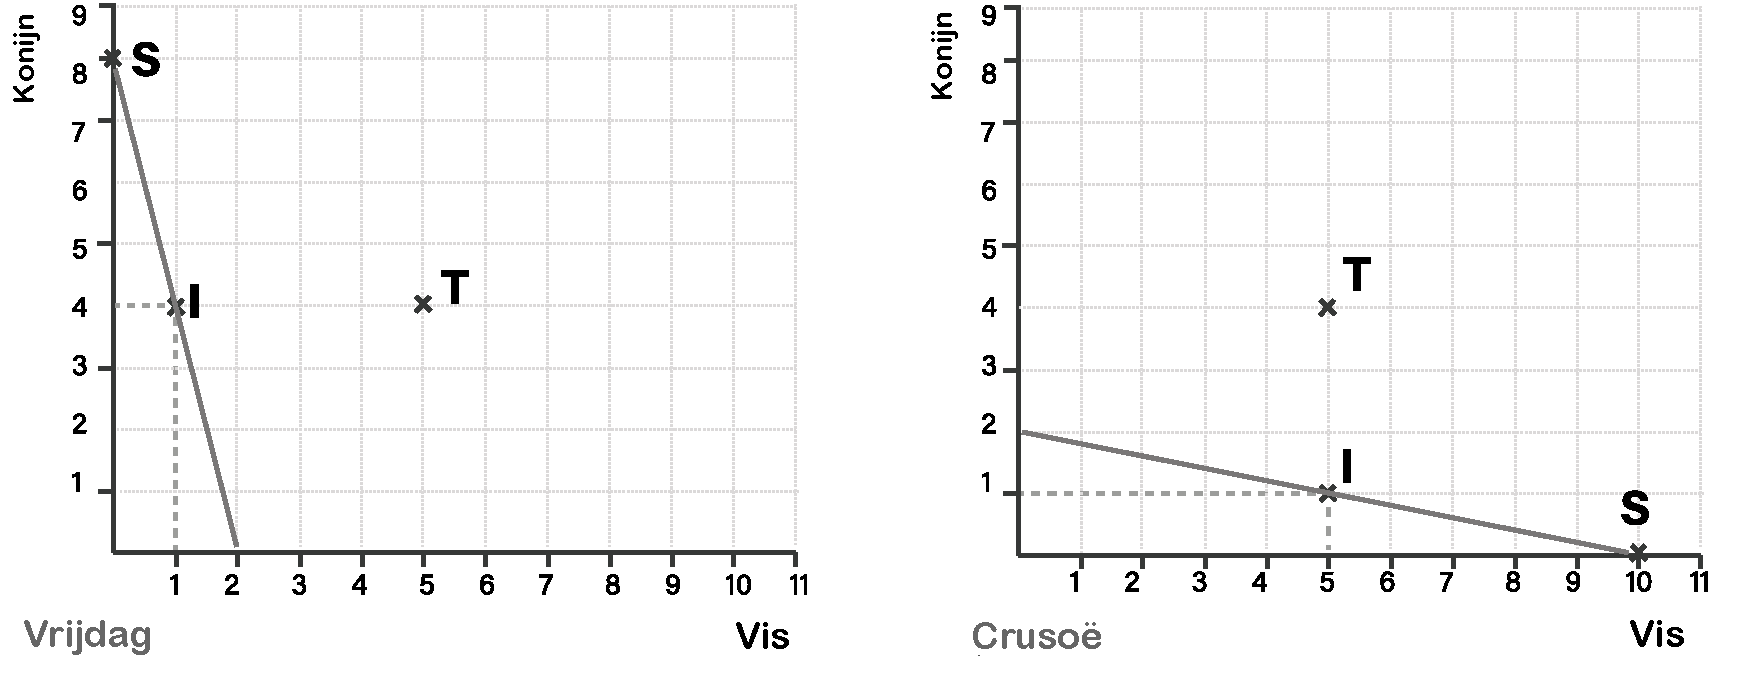
\includegraphics[width=\textwidth]{figures/fig17.pdf}
    \caption[Productiemogelijkheden in isolatie en in handel.]{Productiemogelijkheden in isolatie en in handel}
    \label{fig17}
\end{figure}

Als Crusoë Vrijdag zou aanvallen en proberen te beroven, zou hij misschien al het voedsel dat Vrijdag heeft kunnen meenemen, maar dan zou Vrijdag verhongeren en zou Crusoë niets anders overhouden dan zijn eigen productie\index{productie}, net als in zijn oorspronkelijke staat. Maar als ze zouden besluiten om samen te werken, zouden ze allebei kunnen profiteren van de verschillen in hun vangsten. Omdat Crusoë merkt dat Vrijdag een overvloed aan konijnen heeft, maar niet veel vis, stelt hij voor om wat van zijn konijnen te ruilen tegen de vis van Crusoë. Konijnen zijn er voor Vrijdag in tegenstelling tot vis in overvloed, dus een vis ruilen voor een konijn is zowel voor hem als voor Crusoë een win-winsituatie.

De ruiltransactie laat Vrijdag inzien dat de beste manier om aan vis te komen is om op konijnen te jagen en die te ruilen voor vis, terwijl Crusoë zich realiseert dat hij meer konijnen kan krijgen door te vissen en de vis te ruilen voor konijnen dan door op konijnen te jagen. Het eindresultaat is dat het logisch is dat ze zich specialiseren in de goederen die ze goedkoper kunnen produceren. Als ze zich specialiseren, en Crusoë alleen vis en Vrijdag alleen konijnen vangt, zoals weergegeven in punt S in Figuur 17, dan zou hun gezamenlijke dagelijkse productie\index{productie} 8 konijnen en 10 vissen zijn, wat 3 konijnen en 4 vissen meer is dan ze zouden hebben gehad als ze vijanden waren gebleven. Als ze hun oogst in tweeën delen, krijgen ze elk 4 konijnen en 5 vissen, zoals te zien is in punt T.

Door zich simpelweg te specialiseren in de productie\index{productie} van het goedkopere goed, hebben ze allebei meer vis en konijnen geproduceerd dan wanneer ze elk hun tijd en inspanning hadden verdeeld over de productie\index{productie} van beide. Dit resultaat lijkt bijna een goocheltruc: ze werken allebei evenveel uren en toch hebben ze uiteindelijk allebei meer konijnen en vis te eten en zijn ze allebei beter af. Dit is geen eenmalig voordeel zoals die van de buit na diefstal, maar een duurzame verbetering in hun leven die kan voortduren zolang ze in goede verstandhouding met elkaar blijven handelen. In feite worden ze elke ochtend wakker met een keuze: samenwerken en meer eten of vijandig zijn en minder eten. Door elke persoon in staat te stellen zijn tijd te besteden aan de productie\index{productie} van het goed dat voor hem minder duur is, verhoogt de handel de productiviteit van beide partijen. Als één van hen de ander had gedood, zou de ``winnaar'' nooit zoveel winnen als wanneer hij vrijwillig met de ander zou samenwerken.

\hypertarget{comparatief-voordeel}{%
\section{Comparatief voordeel}\label{comparatief-voordeel}}

De redenering achter absoluut voordeel\index{absoluut voordeel} is intuïtief en gemakkelijk te begrijpen. Elk individu specialiseert zich in wat hij tegen lagere kosten kan produceren, wat leidt tot meer productie\index{productie} van alle goederen. Maar het concept van comparatief voordeel\index{comparatief voordeel} is een meer algemene en krachtige verklaring van de voordelen van handel als gevolg van verschillen in de opportuniteitskosten van goederen, ongeacht de aard en omvang van de verschillen in productiviteit tussen de deelnemers. Ruilhandel kan wederzijds voordelig zijn, zelfs als het ene individu productiever is in de productie\index{productie} van beide betrokken goederen dan de andere persoon, vanwege de verschillen in opportuniteitskosten van goederen voor beide individuen. Het feit dat menselijke tijd het ultieme schaarse goed is, betekent dat samenwerking tussen twee mensen voordelig is voor hen beiden, zelfs als de ene productiever is in het produceren van beide goederen, omdat hun samenwerking hen in staat stelt hun schaarse tijd daar in te zetten waar die het meest productief is.

Stel je voor dat Crusoë in het bovenstaande voorbeeld productiever zou zijn in zowel vissen als jagen, en hij 6 konijnen of 12 vissen per dag zou kunnen produceren, terwijl Vrijdag slechts 4 konijnen of 2 vissen zou kunnen produceren. Dit betekent niet dat de twee geen voordeel kunnen halen uit de arbeidsdeling\index{arbeidsdeling}. Als de twee mannen geïsoleerd hadden geproduceerd en geconsumeerd, en ieder de helft van de dag hadden gejaagd en de andere helft gevist, dan zou Crusoë 3 konijnen en 6 vissen hebben, terwijl Vrijdag 2 konijnen en 1 vis zou hebben, voor een totaal van 5 konijnen en 7 vissen. Als ze samenwerken en zich specialiseren, vangt Vrijdag 4 konijnen en Crusoë 12 vissen, zoals te zien is in punt S. Als ze liever meer konijnen hebben, zou Crusoë een deel van zijn dag kunnen besteden aan jagen, en zouden ze uiteindelijk 5 konijnen en 10 vissen hebben, zoals te zien is in punt S2. In dit geval zouden ze 3 vissen aan hun dagelijkse consumptie\index{consumptie} hebben toegevoegd door zich te specialiseren. Er zijn verschillende andere combinaties van vis en konijnen die ze zouden kunnen produceren, afhankelijk van hun smaak en voorkeur voor beide. Zolang de specialisatie elke producent in staat stelt om zich te concentreren op het goed met de laagste opportuniteitskosten, zouden ze een subjectief waardevollere productie\index{productie} hebben dan wanneer ze individueel zouden produceren.

\begin{figure}[!htb]
\centering
    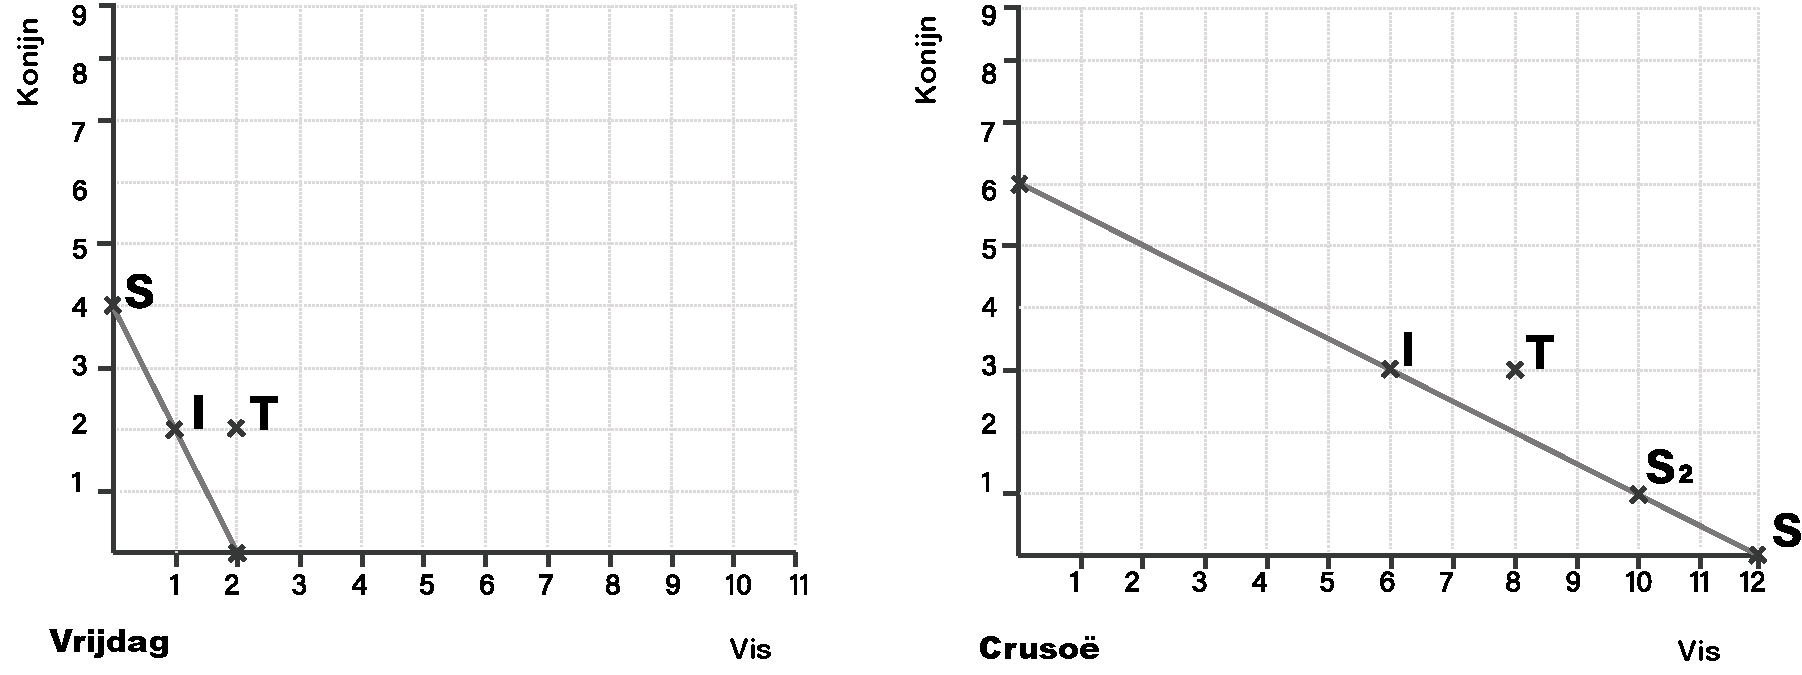
\includegraphics[width=\textwidth]{figures/fig18.pdf}
    \caption[Productiemogelijkheden in isolatie en met comparatief handelsvoordeel]{Productiemogelijkheden in isolatie en met comparatief handelsvoordeel}
    \label{fig18}
\end{figure}

Zowel Crusoë als Vrijdag zouden precies evenveel uren werken, en toch zouden ze meer produceren dan voorheen, ook al is Crusoë productiever in zowel jagen als vissen. Het feit dat de twee mannen verschillende opportuniteitskosten hebben voor de twee goederen betekent dat ze de hoeveelheid die ze produceren kunnen verbeteren door elk meer tijd te besteden aan het produceren van het goed waarvoor ze de lagere opportuniteitskosten hebben. Omdat iedereen zijn tijd besteedt aan het produceren van het goed met de lagere opportuniteitskosten, produceren ze meer van de eindproducten die ze allebei willen.

De specialisatie in dit voorbeeld gebeurt, omdat de opportuniteitskosten van een konijn voor Crusoë gelijk staan aan 2 vissen, terwijl het voor Vrijdag een halve vis is. Deze opportuniteitskosten worden grafisch uitgedrukt als de helling van de productiemogelijkhedengrenscurve. Voor elke periode waarin Crusoë 1 konijn moet bemachtigen, moet hij de tijd opgeven die nodig is om 2 vissen te bemachtigen. Maar Vrijdag heeft andere opportuniteitskosten. Hij kan twee keer zoveel konijnen als vissen produceren in een bepaalde periode. Hij hoeft dus maar een halve vis op te geven om een extra konijn te krijgen. Als iemand Vrijdag een hele vis zou aanbieden in ruil\index{ruil} voor 1 konijn, zou hij die graag aannemen. Op dezelfde manier geldt dat als Vrijdag een konijn zou aanbieden aan Crusoë in ruil\index{ruil} voor een vis, dat Crusoë het aanbod graag zou willen aannemen, omdat dit voor Crusoë een goedkopere manier is om het konijn te krijgen dan het zelf te produceren.

Crusoë heeft twee mogelijkheden om een extra konijn te bemachtigen: 1) minder tijd besteden aan vissen en daarmee 2 vissen opgeven om genoeg tijd te hebben om op 1 konijn te jagen, of 2) Vrijdag iets meer dan een halve vis geven om hem over te halen een van zijn konijnen af te staan. De eerste methode kost Crusoë 2 vissen, terwijl de tweede hem een bedrag kost dat groter is dan een halve vis. Uit eigenbelang kiest Crusoë ervoor om met Vrijdag samen te werken, en dezelfde redenering stimuleert Vrijdag om met Crusoë samen te werken. Alleen al het bestaan van verschillen in opportuniteitskosten tussen de twee betekent dat ze met elkaar kunnen afstemmen om hun eigen arbeid te verdelen op een manier die de totale output maximaliseert, op basis van de voorwaarden die ze aanvankelijk overeenkwamen. Het verschil in opportuniteitskosten is de advertentie voor ruilhandel\index{ruilhandel}. Voor beide personen geeft dit aan dat de ander in staat is te voorzien in zijn of haar behoeftes tegen lagere kosten. Door te streven naar optimalisatie van de eigen productie\index{productie} met het oog op handel, verhoogt dit de productiviteit voor beide partijen.

Ongeacht het verschil in productiviteit tussen de twee, betekent het verschil in opportuniteitskosten dat handel de arbeidsdeling\index{arbeidsdeling} tussen de twee zal veranderen om een grotere output te creëren. Deze handelsmogelijkheden ontstaan in de echte wereld zonder dat economen ze hoeven te bestuderen en uit te werken voor individuen die handel drijven. Als mensen met elkaar omgaan, merken ze dat ze goederen verschillend waarderen. Deze verschillen bieden mogelijkheden voor handel waar beide partijen van profiteren. De logica is van toepassing op het niveau van individuen in een gezin, dorp, stad, land of tussen landen. Verschillen in de opportuniteitskosten van productie\index{productie} bieden kansen voor specialisatie en mensen proberen er voortdurend voordeel uit te halen.

De verschillen in voorkeuren en productiviteit zijn de drijvende krachten achter het overal aanwezige fenomeen van handel. De wiskundige voorbeelden zijn in dit opzicht nuttig, maar ze krijgen te veel nadruk in het moderne economische onderwijs\index{onderwijs}, tot het punt waarop cursussen over internationale handel weinig economisch\index{economisch} inzicht bevatten en in plaats daarvan gericht zijn en toetsen op wiskundige bewerkingen die raakvlakken hebben met deze onderwerpen. De diepgaande inzichten in de voordelen van handel worden meestal slechts kort behandeld in de eerste hoofdstukken van de meeste tekstboeken, terwijl de nodeloos ingewikkelde wiskundige modellen centraal staan. De wiskundige spitsvondigheden maken gestandaardiseerde toetsen makkelijker en veranderen deze leerboeken ook in een reeks uitgebreide, halfbakken rationalisaties voor overheidsinterventie in de handel. Terwijl het gemiddelde economieleerboek begint met een lofzang over vrije handel, ontaardt het al snel in het recyclen van oude mercantilistische onzin door deze via irrelevante wiskundige modellen binnen te smokkelen.

\hypertarget{specialisatie-en-arbeidsverdeling}{%
\section{Specialisatie en arbeidsdeling\index{arbeidsdeling}}\label{specialisatie-en-arbeidsverdeling}}

\begin{blockquotebox}
    Het bestaan en de mogelijkheden van ruilhandel\index{ruilhandel} openen voor producenten de weg om voor een ``markt'' te produceren in plaats van voor zichzelf. In plaats van ieder voor zich te streven naar maximalisatie van de productie\index{productie} door uitsluitend goederen voor eigen gebruik te maken, kan men nu goederen produceren in afwachting van hun marktwaarde, om deze vervolgens in te ruilen voor andere goederen die men waardevoller acht. Het is duidelijk dat aangezien dit een nieuwe weg opent voor het nut van goederen, het voor iedereen mogelijk wordt om zijn productiviteit te verhogen.\footnotemark
    \par\raggedleft--- Murray Rothbard\index{Murray Rothbard}
\end{blockquotebox}
\footautocite{106}

De motivaties voor handel kunnen worden afgeleid uit verschillen in smaak en waardering, zoals hierboven vermeld, maar in een uitgebreide marktorde worden ze uiteindelijk aangewakkerd door verschillen in productiekosten en versterkt door specialisatie.

Terwijl een geïsoleerd individu produceert wat hij nodig heeft, produceert de mens in een sociaal systeem op basis van wat hij verwacht dat anderen nodig hebben. Hij hoeft niet in al zijn behoeften te voorzien door middel van zijn eigen arbeid en kan in plaats daarvan zijn arbeid richten op de productiegebieden waarin hij het meest kan uitblinken in het dienen van anderen. Door zich te specialiseren in het produceren van een goed voor een markt, in plaats van te produceren voor eigen consumptie\index{consumptie}, wordt het mogelijk om arbeid te richten op de plaats waar het het meest productief is, niet waar het alleen maar nodig is. In een markteconomie worden je behoeften het best indirect vervuld, door je te specialiseren in wat je het beste kunt en dit te ruilen voor goederen en diensten die door anderen worden geproduceerd. Specialisatie is daarom een andere manier om de productiviteit te verhogen. Naast een verhoging van de productiviteit leidt handel ook tot sociale samenwerking en beschaafd gedrag, omdat de voordelen van het vreedzaam kunnen deelnemen aan de samenleving in een arbeidsdeling\index{arbeidsdeling} erg groot zijn.

In \textit{Human Action} legt Mises uit dat specialisatie gedreven wordt door verschillen in vaardigheden en door de natuur gegeven factoren. In \textit{Man, Economy, and State} stelt Rothbard dat specialisatie aangejaagd wordt door (a) verschillen in geschiktheid en rendement van de door de natuur gegeven factoren; (b) verschillen in beschikbaar kapitaal\index{kapitaal} en duurzame consumptiegoederen\index{consumptiegoed}; en (c) verschillen in vaardigheid en in de vraag naar verschillende soorten arbeid.

Rothbards uitleg is hier uitgebreider dan die van Mises, en men kan zelfs verder gaan dan Rothbard en stellen dat, vooral in de moderne economie, het met name de accumulatie van kapitaal\index{kapitaal} is die specialisatie aanmoedigt.

In de bovenstaande voorbeelden gingen we ervan uit dat er grote verschillen waren in de productiviteit van jagen en vissen tussen Crusoë en Vrijdag. Maar in de echte wereld worden deze verschillen waarschijnlijk veroorzaakt door verschillen in het beschikbare kapitaal\index{kapitaal}. Crusoë zal een hogere productiviteit hebben bij het vangen van vis omdat hij geïnvesteerd heeft in het maken van een hengel en het bouwen van een vissersboot, terwijl Vrijdag beter zal zijn in het vangen van konijnen omdat hij geïnvesteerd heeft in het maken van vallen en speren. De verschillen in productiviteit zullen waarschijnlijk niet erg groot zijn zonder verschillen in kapitaalvoorraad. Naarmate de technologische vooruitgang en de kapitaalaccumulatie zich in de loop van de tijd hebben ontwikkeld, zijn ze steeds meer los komen te staan van de natuurlijke omstandigheden, en als zodanig worden de productiviteit en het comparatieve voordeel in deze sectoren voornamelijk bepaald door de mate van fysieke en menselijke kapitaalaccumulatie.

Het is logisch dat geografische en natuurlijke factoren een grote rol spelen bij het bepalen van het comparatieve voordeel in landbouw- en natuurproducten. Finland zal zich waarschijnlijk nooit specialiseren in de productie\index{productie} van tropisch fruit zoals mango\textquotesingle s en de Sahara zal waarschijnlijk geen drinkwater exporteren. In een moderne geïndustrialiseerde economie maken deze soorten producten echter een steeds kleiner deel uit van zowel de economische activiteit als de persoonlijke uitgaven van iedereen, in vergelijking met diensten en industriële goederen. In de moderne economie is de drijvende kracht achter specialisatie grotendeels de investering van kapitaal\index{kapitaal} in een industrie. Plaatsen die decennialang hebben geïnvesteerd in autoproductie, hebben het fysieke en menselijke kapitaal\index{kapitaal} ontwikkeld dat geschikt is voor de autoproductie, en zullen waarschijnlijk een voordeel blijven halen uit autoproductie. Plaatsen die investeren in een infrastructuur voor de textielindustrie zullen waarschijnlijk voordelig blijven ontwikkelen. Naarmate de economie geavanceerder wordt en de productiestructuren complexer, wordt comparatief voordeel\index{comparatief voordeel} steeds meer het resultaat van verschillen in kapitaalaccumulatie en minder van verschillen in natuurlijke omstandigheden.

De industrie met de hoogste productiviteit in de moderne wereld is waarschijnlijk de computer- en telecommunicatie-industrie, die een enorme toename van de productiviteit blijft realiseren, terwijl het alle industrieën binnendringt en veel efficiënter maakt. Het concurrentievermogen in deze industrie staat bijna volledig los van natuurlijke en geografische factoren. De software-ingenieurs en programmeurs in deze industrie hebben alleen de kapitaalinfrastructuur nodig om te kunnen produceren, ongeacht of ze dat doen op een tropisch eiland als Singapore of in een bevroren Arctisch landschap zoals het noorden van Zweden. Dit is nog een reden waarom ik geloof dat de moderne economische wetenschap zich te weinig richt op het belang van kapitaalaccumulatie en te veel belang hecht aan handel en arbeidsdeling\index{arbeidsdeling} op zichzelf. Zonder aanzienlijke kapitaalaccumulatie zou er weinig ruimte zijn voor de productiviteitsstijgingen die de verschillen in opportuniteitskosten aandrijven, wat specialisatie noodzakelijk maakt.

Handel is een fenomeen dat op natuurlijke wijze ontstaat wanneer mensen met elkaar in contact komen en zich realiseren dat ze verschillende goederen verschillend waarderen. Als ze zich beginnen te realiseren dat ze meer in hun behoeften kunnen voorzien door voor de markt te produceren dan door rechtstreeks voor hun behoeften te produceren, raken mensen meer gericht op de behoeften van de markt en beginnen ze hun productiecapaciteit af te stemmen op het voorzien in de behoeften van de samenleving. Dit leidt tot een maatschappelijke arbeidsdeling\index{arbeidsdeling}, waarbij werk wordt verdeeld onder de bevolking. Hoe meer individuen zich kunnen specialiseren in de productie\index{productie} van een goed, hoe meer ze na verloop van tijd hun productiviteit zullen verbeteren.


\hypertarget{marktomvang}{%
\section{Marktomvang}\label{marktomvang}}

\begin{blockquotebox}
    Elke stap richting een verder ontwikkelde arbeidsdeling\index{arbeidsdeling} dient de belangen van alle deelnemers ... De factor die de primitieve samenleving tot stand bracht en dagelijks toewerkt naar haar voortdurende intensivering is het menselijk handelen\index{menselijk handelen}, wat gestimuleerd wordt door het besef van de hogere arbeidsproductiviteit die bereikt wordt onder een arbeidsdeling\index{arbeidsdeling}.\footnotemark
    \par\raggedleft--- Ludwig von Mises\index{Ludwig von Mises}
\end{blockquotebox}
\footautocite{107}

In de vorige paragrafen bekeken we het voorbeeld van twee mannen op een geïsoleerd eiland die voordeel haalden door met elkaar te handelen en zich te specialiseren in de productie\index{productie} van de goederen waarvoor ze de laagste opportuniteitskosten hadden. Dit eenvoudige voorbeeld illustreert de beweegredenen voor handel en de stimulerende krachten achter de voordelen van handel, maar dezelfde logica geldt als het aantal handelspartners in de loop der tijd toeneemt en de winsten alleen maar toenemen naarmate het aantal partners toeneemt. Dit komt doordat diepere specialisatie meer kapitaalaccumulatie en een hogere productiviteit mogelijk maakt.

In de eenpersoonseconomie moet Crusoë zelf in al zijn behoeften voorzien. Met het jagen, het bouwen van een huis, het maken van wapens om roofdieren te bestrijden en het maken van zijn eigen kleren, heeft hij nauwelijks tijd om alle noodzakelijke taken uit te voeren. Hij heeft heel weinig ruimte voor specialisatie en heel weinig tijd om kapitaalgoederen\index{kapitaalgoederen} te ontwikkelen in één bepaalde richting van productie\index{productie} omdat hij zijn tijd moet verdelen tussen vele taken. Met een andere man op het eiland kunnen beiden zich specialiseren in de helft van de taken en hun producten verhandelen. Slechts één van hen hoeft te vissen, terwijl de ander zich richt op de jacht. De jager kan nu twee keer zoveel tijd besteden aan het ontwikkelen van speren en vallen, terwijl de visser twee keer zoveel tijd kan besteden aan het maken van vishengels en boten. Omdat ze nu allebei de helft minder taken hebben, kunnen ze meer tijd besteden aan elke missie en er dus beter in worden en er meer kapitaal\index{kapitaal} voor opbouwen. De mate van kapitaalaccumulatie en specialisatie neemt alleen maar toe naarmate meer mensen deelnemen aan de markt en met elkaar handelen.

Als Crusoë en Vrijdag nog eens 20 mensen op het eiland zouden tegenkomen, dan zou de mogelijkheid voor specialisatie nog groter worden. Nu zou slechts één persoon zich specialiseren in het bouwen van huizen, terwijl een ander zich zou richten op landbouw, een ander op kleding, weer een ander op jagen, weer een ander op het maken van vishengels en weer een ander op het maken van speren voor de jacht. Dezelfde logica van verhoogde productie\index{productie} die we zagen toegepast op Crusoë en Vrijdag kan nu worden toegepast op deze grotere groep, met een continu toenemende productiviteit.

Het vergroten van de marktomvang verhoogt niet alleen de productiviteit van werknemers, maar het verhoogt ook het aantal en de verscheidenheid aan goederen die beschikbaar zijn voor deelnemers aan de samenleving. Naarmate het aantal mensen op de markt toeneemt en de productiviteit van individuele producenten stijgt, kan elke producent van elk goed genoeg produceren om in de behoeften van een toenemend aantal mensen te voorzien. Dit maakt arbeiders vrij om nieuwere, innovatieve goederen te produceren die verder gaan dan de meest elementaire behoeften.

Naarmate de cirkel waarbinnen iemand handelt groter wordt, nemen de productiviteit en de hoeveelheid beschikbare goederen toe. Deze observatie van de marktomvang is een zeer krachtig hulpmiddel om economische verschijnselen te verklaren. Het helpt om de economische drijfveer voor immigratie van het platteland naar de grote steden te verklaren. Een arbeider in een geïsoleerd plattelandsgebied produceert voor een kleine kring van potentiële kopers en koopt van een kleine kring van producenten. Hij moet in veel van zijn eigen behoeften voorzien omdat er geen professionele aanbieders van deze diensten zijn. Hij moet een deel van zijn werkdag besteden aan het produceren van dingen waarvoor geen specialisten in zijn omgeving zijn, waarin hij niet gespecialiseerd is en waarin zijn productiviteit relatief laag is. Als hij bijvoorbeeld schoenmaker zou zijn, zou hij verantwoordelijk zijn voor alle productiefasen van de schoen, inclusief het ontwerp en het samenstellen van de onderdelen, en ook voor de zool, veters en het comfort. Maar als hij naar een grote stad verhuist, kan hij zich specialiseren in het aspect van deze processen waar hij het meest bedreven in is en waar zijn productiviteit het hoogst is. Hij kan voor de overige taken een beroep doen op anderen. Hij kan zich richten op de assemblage van de schoen, terwijl hij gebruik maakt van de ontwerpen van gespecialiseerde en zeer productieve ontwerpers, en de veters en zolen kopen van specialisten die ze maken tegen veel lagere kosten dan hij zelf zou kunnen. De schoenmaker kan in een grote stad meer verdienen en productiever zijn dan in een kleine geïsoleerde plattelandsstad.

In een wereld die is opgedeeld in geïsoleerde economieën van 1.000 mensen elk, kunnen er geen auto\textquotesingle s, computers of smartphones zijn. De 1.000 mensen zouden zich bezighouden met het produceren voor hun basisbehoeften. Als deze geïsoleerde gemeenschappen met elkaar gaan handelen, neemt de mate van specialisatie toe en kan de kapitaalaccumulatie in elk productieproces\index{productieproces} toenemen, waardoor meer mensen zich kunnen losmaken van arbeid gericht op basaal overleven zodat ze zich kunnen richten op de productie\index{productie} van kapitaalgoederen\index{kapitaalgoederen} die niet direct consumptiegoederen\index{consumptiegoed} opleveren. Naarmate de marktomvang toeneemt, nemen de beloningen van specialisatie toe, omdat de producten aan grotere groepen mensen verkocht kunnen worden. De huidige wereldmarkt is de grootste markt die ooit heeft bestaan en maakt het hoogste productiviteitsniveau mogelijk dat ooit is bereikt.

De technologisch geavanceerde producten die we vandaag de dag gebruiken zouden simpelweg niet mogelijk zijn in een wereld met 1\% van de huidige bevolking, of een wereld van kleine, afgezonderde markten\index{markten}. Om een moderne autofabriek in staat te stellen om het aantal auto\textquotesingle s te produceren dat het vandaag de dag tegen de huidige prijzen kan produceren, is een groot aantal mensen nodig die gespecialiseerd zijn in steeds specifiekere en ingewikkelder taken, die alleen mogelijk zijn als een groot aantal auto's aan grote markten\index{markten} kan worden verkocht. Een moderne autofabrikant heeft ingenieurs die zich vele jaren focussen op zeer kleine details van de productie\index{productie} van een auto, zoals een voorruit. Zonder de mogelijkheid voor de autofabrikant om auto\textquotesingle s aan grote markten\index{markten} te verkopen, zou de mate van specialisatie noodzakelijkerwijs afnemen en daarmee ook de verfijning en waarde van het product en de productiviteit van de werknemers.

Het is echt een wonder als je denkt aan de mate van specialisatie van taken die nodig zijn om moderne producten te maken. In een beroemd essay probeert Leonard Read de mate van samenwerking te schetsen die nodig is om een modern potlood te maken.\autocite{108} Ook al heeft een fabriek het potlood in elkaar gezet en geproduceerd, er is niet één mens die weet hoe hij het potlood vanaf nul moet maken. De fabriek die het potlood in elkaar zette was slechts één stadium van een lang productieproces\index{productieproces} waarbij talloze gespecialiseerde mensen wereldwijd betrokken zijn. Van het snijden van het hout, tot het verwerken van het rubber dat in de gum gaat, tot de metalen die in de houder van de gum gaan, talloze individuen moeten samenwerken om elk van deze materialen in hun ruwe vorm te krijgen, ze te vervoeren naar de fabrieken waar ze verwerkt werden, en ze om te zetten in de producten die de potlodenfabriek kan gebruiken. Deze arbeidsdeling\index{arbeidsdeling} is alleen mogelijk door de grote markt waarin deze producenten handelen. Als al deze mensen zouden besluiten om geen handel te drijven met de wereld, dan zouden ze al hun dagen besteden aan enkel te overleven. Door samen te werken en handel te drijven, zijn ze in staat zich te specialiseren in de productie\index{productie} van zeer geavanceerde goederen, met een hoge productiviteit, en de producten van de specialisatie van anderen tegen zeer lage kosten te consumeren. De extreem complexe productie\index{productie} van potloden wordt over de hele wereld geregeld zonder één centrale planner die op de hoogte is van alle details. De output bestaat uit tientallen miljarden potloden die elk jaar worden geproduceerd en beschikbaar zijn tegen steeds lagere prijzen.

Naarmate de markt waarmee een individu handel kan drijven groter wordt, kan hij kiezen uit een groeiend aantal producenten en verkopen aan een groeiend aantal consumenten. Hij kan zich specialiseren in steeds specifiekere taken, waardoor de arbeidsdeling\index{arbeidsdeling} toeneemt en er steeds geavanceerdere producten worden ontwikkeld. Hij is in staat om steeds grotere hoeveelheden kapitaal\index{kapitaal} te verzamelen om zijn taak uit te voeren en zo een steeds hogere productiviteit te bereiken. De beste markt waarmee een individu handel kan drijven is de grootst mogelijke markt: de hele wereld. Individuen die leven in landen met geen of lage handelstarieven zijn in staat om hun productiviteit te verhogen door zich te specialiseren in zeer specifieke taken die ze kunnen verkopen aan de hoogste bieder ter wereld, en ze zijn in staat om hun levensstandaard te verhogen door voor zichzelf de beste en meest betaalbare producten te kiezen van producenten over de hele wereld.

Dit inzicht helpt ons ook te begrijpen waarom productiviteit, inkomen en levenskwaliteit toenemen naarmate een samenleving beter geïntegreerd raakt in de wereldhandel. Het piepkleine eiland Sint-Helena ligt in de Zuid-Atlantische Oceaan, 1.950 kilometer ten westen van Kaapstad en 4.000 kilometer ten oosten van Rio de Janeiro, en heeft ongeveer 6.000 inwoners. Handel drijven met de rest van de wereld is erg duur voor de inwoners van Sint-Helena omdat er hoge transportkosten mee gemoeid zijn. Al het kapitaal\index{kapitaal} dat wordt geïmporteerd naar Sint-Helena zal erg duur zijn, waardoor binnenlandse productie\index{productie} duurder is dan in beter geïntegreerde locaties. Ingevoerde consumptiegoederen\index{consumptiegoed} zijn duur voor de inwoners van Sint-Helena vanwege de handelskosten, en hun export naar de rest van de wereld zal gepaard gaan met hoge kosten.

We kunnen een gelijkaardig patroon waarnemen wanneer overheidsambtenaren een beleid invoeren dat hun land in feite vergelijkbaar maakt met het afgezonderde Sint-Helena, namelijk handelsbeperkingen. Door handelstarieven op te leggen, verhogen regeringen de kosten van handel met de rest van de wereld, waardoor de markt voor individuen in hun land kleiner wordt. De goederen uit de rest van de wereld worden duurder en de mogelijkheden om te specialiseren worden beperkt. Tot de meest geïsoleerde economieën op aarde behoren Noord-Korea, Cuba, Eritrea en Venezuela. Het zal geen verrassing zijn dat de productiviteit en levensstandaard in deze economieën erg laag zijn. In het verleden, toen Venezuela een vrijemarkteconomie was die openstond voor de wereld, had het een van de hoogste levensstandaarden ter wereld.

Aan de andere kant van Sint-Helena en de isolationistische economieën staan de economieën met de meest vrije handel ter wereld, waarvan de burgers handel kunnen drijven met een zeer grote wereldmarkt, ongeacht de omvang van hun eigen economie. Burgers van Hongkong, Singapore, Nieuw-Zeeland en Zwitserland ondervinden de minste belemmeringen om te handelen met de rest van de wereld waardoor de productiviteit en levensstandaard van hun inwoners tot de hoogste ter wereld behoren. Wanneer een burger van een geïsoleerde economie een goed wil kopen, kan hij dat alleen bij binnenlandse producenten kopen. Wanneer de burger van een open economie hetzelfde goed wil kopen, kan hij wereldwijd producten kiezen. Burgers van een open economie kunnen veel productiever zijn omdat ze productieprocessen kunnen uitvoeren die aan de hele planeet verkopen, meer inkomsten genereren en meer investeringen mogelijk maken om het productieproces\index{productieproces} te verlengen en geavanceerder te maken.

De afwezigheid van handelsrestricties tussen de jonge Amerikaanse staten stimuleerde de economische opkomst van de Verenigde Staten\index{Verenigde Staten} aanzienlijk. Bovenop de relatief lage tarieven voor internationale handel, stelde vrijhandel in Noord-Amerika een zeer grote bevolking in staat om onderling handel te drijven met toenemende specialisatie. Tegen het einde van de negentiende eeuw was de VS qua bevolking het grootste land van alle westerse economieën die in die eeuw industrialiseerden, waardoor het een aanzienlijk economisch\index{economisch} voordeel had en meer specialisatie en een hogere productiviteit mogelijk maakte. Als er handelsbarrières waren opgericht tussen verschillende staten, is het zeer onwaarschijnlijk dat de VS economisch\index{economisch} zoveel vooruitgang zou hebben geboekt.

Economie als wetenschap probeert de alom aanwezigheid van handel te verklaren. Het is geen wonder dat mensen voortdurend proberen om handel met elkaar te drijven. Het moedigt mensen aan om hun agressieve en vijandige instincten ten opzichte van anderen te matigen en in plaats daarvan te streven naar productieve samenwerking. Het als vreemden zonder verbondenheid via een familie of kennissenkring tot een wederzijds voordelige ruil\index{ruil} te komen, is een van de fundamentele bouwstenen van de menselijke beschaving\index{beschaving}. De mate waarin onbekenden kunnen verwachten vreedzaam met elkaar om te gaan, met respect voor elkaars lichaam, eigendom en vrije wil, is de indicator van hoe beschaafd een maatschappij is.
